\newvideofile{OPV_Schaltungen}{Schaltungen}
\begin{frame}
    \b{
        \fta{Prinzip der Gegenkopplung}
        Es soll ein Leistungsverstärker aufgebaut werden, der geeignet ist, das Signal eines Handys so zu verstärken, dass ein Lautsprecher damit betrieben werden kann.
        Das Eingangsspannungsniveau ist 1\,V und es soll ein 4\,$\mathrm{\Omega}$ Lautsprecher betrieben werden.
        Wie groß muss die Spannung am Ausgang des Verstärkers sein, damit der Lautsprecher bei 1\,kHz 25\,W aufnimmt.
        Wie kann hier vorgegangen werden, wenn eine Operationsverstärkerschaltung für die Lösung genutzt werden soll? \par
        \fu{\resizebox{0.8\textwidth}{!}{\input{Tikz/src/OPVBeispielproblem.tex}}}{Schaltung des Beispielproblems mit einer Signalquelle auf der Eingangsseite und einer komplexen Last auf der Ausgangsseite \label{fig:Beispielproblem 1 Folien}}.
    }
    \speech{Gegenkopplung}{1}{In den vorherigen Videos haben wir uns auf den inneren Aufbau des Verstärkers seine charakteristischen Größen konzentriert. Nun schauen wir uns die Beschaltungsmöglichkeiten an.
        Starten wir mit einer kleinen Motivation: Angenommen, wir wollen ein Musiksignal von unserem Handy über einen Lautsprecher wiedergeben. Das Handy liefert vielleicht eine Spannung von rund einem Volt.
        Der Lautsprecher braucht aber 25\,Watt an 4\,Ohm - das entspricht einer Ausgangsspannung von ungefähr zehn Volt.
        Wir brauchen also eine Schaltung, die diese Verstärkung übernimmt - einen Verstärker.}
    %seed: 875677
    \silence{3}
\end{frame}

\begin{frame}
    \s{
        \fta{Prinzip der Gegenkopplung}
        Nachdem die vorherigen Kapitel zunächst den inneren Aufbau des Verstärkers und das sich daraus ergebenden Modell sowie die im idealen Modell nicht beschriebenen, realen Effekte thematisierten, soll es in diesem Unterkapitel um die Beschaltung des Operationsverstärkers gehen.
    
        Es sollen im Rahmen dieses Kapitels folgende Kompetenzen erworben werden:
        \s{
            \begin{Lernziele}{Operationsverstärker}
                \title{Lernziele: Prinzip der Gegenkopplung}
                Die Studierenden können
                \begin{itemize}
                    \item verschiedene Operationsverstärkerschaltungen und mögliche Einsatzgebiete nennen.
                    \item die Funktion von vorliegenden Operationsverstärkerschaltungen bestimmen und mithilfe der Kirchhoff'schen Gesetze die Verstärkung berechnen.
                    \item wichtige Eigenschaften von Operationsverstärkerschaltungen benennen.
                \end{itemize}
            \end{Lernziele}
        }
    
        Dazu soll ein Problem dargestellt werden, für dessen Lösung ein Operationsverstärker verwendet werden soll. Anhand dieses Problems soll die Verwendung von Operationsverstärkern Schritt für Schritt motiviert werden. \par
        \begin{bsp}{ Teil 1: Entwicklung einer Verstärkerschaltung für Musiksignale}{ Beispiel Verstaerkung }
            Bei der Entwicklung von Hi-Fi-Geräten müssen Verstärker an die Last (also den Lautsprecher) angepasst werden.
            Dazu wird ein Leistungsverstärker (d.h. eine Endstufe) benötigt. Eine solche Endstufe, die geeignet ist, das Signal eines Handys so zu verstärken, dass ein Lautsprecher damit betrieben werden kann soll hier aufgebaut werden.
            Ein vereinfachtes Ersatzschaltbild des Lautsprechers ist durch eine Induktivität mit einem in Reihe geschalteten Widerstand gegeben (siehe Abbildung \ref{fig:Beispielproblem 1}).
            Das Eingangsspannungsniveau ist $1\,\mathrm{V}$ und es soll ein $4\,\Omega$ Lautsprecher betrieben werden ($4\,\Omega$ bedeutet, dass der Lautsprecher bei $1\,\mathrm{kHz}$ eine Impedanz von $4\,\Omega$ aufweist).
            Wie groß muss die Spannung am Ausgang des Verstärkers sein, damit der Lautsprecher bei $1\,\mathrm{kHz}$ $25\,\mathrm{W}$ aufnimmt.
            Wie kann hier vorgegangen werden, wenn eine Operationsverstärkerschaltung für die Lösung genutzt werden soll? \par
    
            \textbf{Lösung}\\
            Zunächst muss dazu die Spannung berechnet werden, die der Verstärker ausgeben soll.
            \begin{equation}
                U_{\textnormal{A}} = \sqrt{P \cdot R} = \sqrt{25\,\mathrm{W} \cdot 4\,\mathrm{\Omega}} = 10\,\textnormal{V}
            \end{equation}
            Wie kann nun mithilfe eines Operationsverstärkers der mit einem \glqq ?\grqq{} gekennzeichneten Teil der Schaltung ersetzt werden, um eine notwendige Verstärkung von 10 zu erreichen (siehe Abbildung \ref{fig:Beispielproblem 1}).
            \fu{\resizebox{0.6\textwidth}{!}{\input{Tikz/src/OPVBeispielproblem.tex}
            \alttext{Die Abbildung zeigt eine elektrische Schaltung zur Ansteuerung eines Lautsprechers.
            Die Abbildung zeigt eine elektrische Schaltung zur Ansteuerung eines Lautsprechers. \(U_{\mathrm{eff}}= 1 \ \mathrm{V}\).Sie ist zwischen zwei Leitungen geschaltet, die nach rechts zu einem rechteckig dargestellten Block führen. In diesem Block steht ein Fragezeichen, was darauf hinweist, dass hier eine unbekannte oder zu bestimmende Schaltung dargestellt ist.
            Rechts davon befindet sich das Ersatzschaltbild eines Lautsprechers, das durch eine gestrichelte Umrandung gekennzeichnet ist. Dieses besteht aus einem Widerstand mit \(2 \ \Omega \), der in Serie mit einer Induktivität von \(100 \ \mathrm{mH}\) geschaltet ist. Die Induktivität ist unten mit Masse verbunden.}}}
            {Schaltung des Beispielproblems mit einer Signalquelle auf der Eingangsseite und einer komplexen Last auf der Ausgangsseite. Es wird für den mit einem Fragezeichen gekennzeichneten Teil der Schaltung zunächst der Verstärkungsfaktor $V=\frac{U_{\textnormal{A}}}{U_{\textnormal{E}}}$ gesucht. \label{fig:Beispielproblem 1}}
        \end{bsp}
    }

    \b{
        \frametitle{Prinzip der Gegenkopplung - Lösung des Beispielproblems (1)}
        \textbf{Lösung}\\
        Zunächst muss dazu die Spannung berechnet werden, die am Ausgang des Verstärkers anliegen soll.
        \begin{equation}
            U_{\textnormal{A}} = \sqrt{P \cdot R} = \sqrt{25\,\mathrm{W} \cdot 4\,\mathrm{\Omega}} = 10\,\textnormal{V}
        \end{equation}
        Wie kann nun mithilfe eines Operationsverstärkers der mit einem \glqq ?\grqq{} gekennzeichneten Teil der Schaltung ersetzt werden, um eine notwendige Verstärkung von 5 zu erreichen.
        \fu{\resizebox{0.8\textwidth}{!}{\input{Tikz/src/OPVBeispielproblem.tex}}}{Schaltung des Beispielproblems mit einer Signalquelle auf der Eingangsseite und einer komplexen Last auf der Ausgangsseite \label{fig:Beispielproblem 1 Folien 2}}
    }
    \speech{Gegenkopplung_Bsp}{1}{Hier sehen wir die einfache Rechnung: Mit 25\,Watt an 4\,Ohm brauchen wir eine Spannung von zehn Volt. Das heißt, wir benötigen eine Spannungsverstärkung von zehn zu eins, also den Faktor zehn. Wie können wir das mit einem Operationsverstärker umsetzen?} 
    %seed: 875681 
    \silence{3}
\end{frame}

\begin{frame}
    \b{
        \frametitle{Prinzip der Gegenkopplung - Lösung des Beispielproblems (2)}
        \begin{center}
            \begin{tabular}{ |>{\centering\arraybackslash}m{0.25\linewidth}|}
                \hline
                \large \textbf{A}                                 \\
                \scalebox{0.8}{    \begin{circuitikz}
        \ctikzset{tripoles/en amp/input height=-0.45}
        \draw (0,0) node[en amp](E){};
        \draw (E.out) node[ocirc]{} node[right]{$U_A$};
        \draw (E.-) node[ocirc]{} node[left]{0\,V};
        \draw (E.+) node[ocirc]{} node[left]{1\,V};
        \draw (E.up) -- ++(0,0.25) node[above]{$+U_\mathrm{B}$} node[ocirc] {};
        \draw (E.down) -- ++(0,-0.25) node[below]{$-U_\mathrm{B}$} node[ocirc] {};
    \end{circuitikz} } \\
                \hline
                \scalebox{1}{    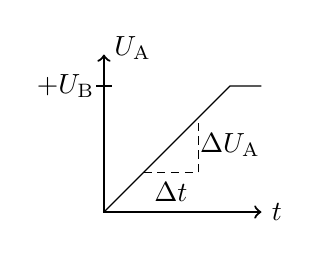
\begin{tikzpicture}
        \draw[thick,->] (-0.015,0) -- (2,0) node[anchor=west] {$t$};
        \draw[thick,->] (0,0) -- (0,2) node[anchor=south west, pos=0.9] {$U_\mathrm{A}$};
        \draw (0,0) -- (1.6,1.6) -- (2,1.6);
        \draw[thick] (-0.1,1.6) -- (0.1,1.6);
        \draw (0,1.6) node[anchor=east] {$+U_\mathrm{B}$};
        
        \draw[densely dashed] (0.5,0.5) -- (1.2,0.5) -- ++(0,0.7);  % Steigungsdreieck Linien
            \node at (1.6,0.85) {$\Delta U_\mathrm{A}$};
            \node at (0.85,0.25) {$\Delta t$}; 
    \end{tikzpicture}
}   \\
                \hline
            \end{tabular}
        \end{center}
    }
    \speech{Gegenkopplung_Bsp_Lsg_1}{1}{Schauen wir uns nun einige Beispiele für Verschaltungsarten an. Wenn wir einen OP V einfach so beschalten, ohne weitere Widerstände und ohne Rückführung, dann arbeitet er wie ein Komparator. Das heißt: Schon eine winzige Differenz zwischen den beiden Eingängen entscheidet darüber, ob der Ausgang auf plus U B oder auf minus U B geht. Man sieht hier auch die Slew Rate, also die maximale Geschwindigkeit, mit der der Ausgang überhaupt ansteigen kann. Kurz gesagt: Ohne Rückkopplung ist der OP V nur als Komparator geeignet, nicht als linearer Verstärker.}
    %seed: 875682 
    \silence{3}
\end{frame}

\begin{frame}
    \b{
        \frametitle{Prinzip der Gegenkopplung - Lösung des Beispielproblems (2)}
        \begin{center}
            \begin{tabular}{ |>{\centering\arraybackslash}m{0.25\linewidth}|>{\centering\arraybackslash}m{0.25\linewidth} >{\centering\arraybackslash}m{0.25\linewidth}| }
                \hline
                \large \textbf{A}                                 &
                \large \textbf{B}                                 &
                \large \textbf{C}                                   \\
    
                \scalebox{0.8}{    \begin{circuitikz}
        \ctikzset{tripoles/en amp/input height=-0.45}
        \draw (0,0) node[en amp](E){};
        \draw (E.out) node[ocirc]{} node[right]{$U_A$};
        \draw (E.-) node[ocirc]{} node[left]{0\,V};
        \draw (E.+) node[ocirc]{} node[left]{1\,V};
        \draw (E.up) -- ++(0,0.25) node[above]{$+U_\mathrm{B}$} node[ocirc] {};
        \draw (E.down) -- ++(0,-0.25) node[below]{$-U_\mathrm{B}$} node[ocirc] {};
    \end{circuitikz} } &
                \scalebox{0.8}{\input{Tikz/src/OPV_Prinzip_Cir2}} &
                \scalebox{0.8}{    \begin{circuitikz}
        \ctikzset{tripoles/en amp/input height=-0.45}
        \draw (0,0) node[en amp](E){};
        \draw (E.out) to[short, -o] ++(0.25,0) node[right]{$U_\mathrm{A}$};
        \draw (E.-) to[short, -o] ++(-0.25,0) node[left]{0\,V}; 
        \draw (E.+) to[short, -o] ++(-0.25,0) node[left]{1V};
        \draw (E.-) to [short, *-] ++(0, -1) to[short] (E.out |- 0,-1.5) to [short, -*] (E.out);
    \end{circuitikz}}   \\
                \hline
                \scalebox{1}{    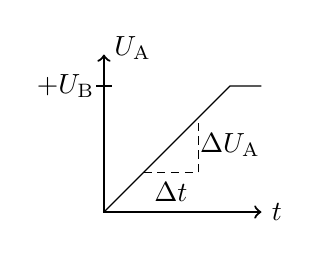
\begin{tikzpicture}
        \draw[thick,->] (-0.015,0) -- (2,0) node[anchor=west] {$t$};
        \draw[thick,->] (0,0) -- (0,2) node[anchor=south west, pos=0.9] {$U_\mathrm{A}$};
        \draw (0,0) -- (1.6,1.6) -- (2,1.6);
        \draw[thick] (-0.1,1.6) -- (0.1,1.6);
        \draw (0,1.6) node[anchor=east] {$+U_\mathrm{B}$};
        
        \draw[densely dashed] (0.5,0.5) -- (1.2,0.5) -- ++(0,0.7);  % Steigungsdreieck Linien
            \node at (1.6,0.85) {$\Delta U_\mathrm{A}$};
            \node at (0.85,0.25) {$\Delta t$}; 
    \end{tikzpicture}
}   &
                Slew rate: $\frac{\Delta U_A}{\Delta t}$          &
                \scalebox{1}{    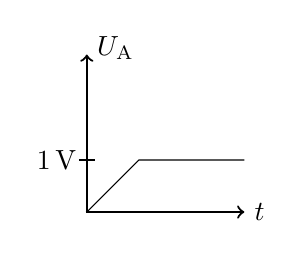
\begin{tikzpicture}
        \draw[thick,->] (-0.015,0) -- (2,0) node[anchor=west] {$t$};
        \draw[thick,->] (0,0) -- (0,2) node[anchor=south west, pos=0.9] {$U_\mathrm{A}$};
        \draw (0,0) -- (0.66,0.66) -- (2,0.66);
        \draw[thick] (-0.1,0.66) -- (0.1,0.66) node[anchor=east, pos=0.5] {$1\,\mathrm{V}$};
    \end{tikzpicture}
}     \\
                \hline
            \end{tabular}
        \end{center}
    }
    \speech{Gegenkopplung_Bsp_Lsg_2}{1}{Wenn wir den Ausgang auf den invertierenden Eingang legen, erzeugen wir eine Rückführung. Das Resultat: Die Ausgangsspannung kann jetzt maximal den Betrag der eingangsseitigen Spannungsdifferenz erreichen. Aber natürlich nur wenn der OP V nicht schon vorher in den Sättigungsbereich kommt. Der OP V versucht nun ständig, die Differenzspannung zwischen plus und minus Eingang auf null zu regeln.}
    %seed: 875683
    \silence{3}
\end{frame}

\begin{frame}
    \s{
        \pagebreak
        Wie aus vorherigen Kapiteln bekannt ist, besitzen Operationsverstärker einen invertierenden und einen nicht-invertierenden Eingang. Existiert zwischen diesen beiden Eingängen eine Spannungsdifferenz, so verstärkt der Operationsverstärker diese Differenz um ein Vielfaches, bis die Spannung die maximale Ausgangsspannung des Operationsverstärkers erreicht (siehe A in Abbildung \ref{fig: Verschaltung Verstaerker}).
        Die Slew-Rate (zu deutsch: Anstiegsrate) gibt an, wie schnell dieser Anstieg geschehen kann. Wird die Ausgangsspannung nicht auf den Eingang zurückgeführt, steigt die Ausgangspannung, bis das Niveau der Versorgungsspannung erreicht wird. Eine solche Beschaltung des Verstärkers wird als Komparatorschaltung bezeichnet.

        Dieses Verhalten ist für die meisten Anwendungen bei denen der Eingangsspannungssignal mit geringer Amplitude verstärkt werden soll, nicht erwünscht.
        Stattdessen werden Operationsverstärker meistens in der sogenannten Gegenkopplung (B) betrieben, bei der der Ausgang auf den invertierenden Eingang zurückgeführt wird.
        Der in (B) eingezeichnete Schalter sei zunächst geöffnet und der Operationsverstärker werde nicht mit Spannung versorgt. Zum Zeitpunkt 0\,s wird der Schalter geschlossen und die Versorgungsspannung des Verstärkers eingeschaltet, wodurch die Rückführung des Ausgangssignals $U_{\textnormal{A}}$ aktiv wird (C).
        Durch die Rückkopplung des Ausgangssignal wird so erreicht, dass die Spannung am invertierenden Eingang auf das Spannungsniveau der Ausgangsspannung angeglichen wird.
        Die in (C) dargestellte Verstärkerschaltung hat die Verstärkung 1 und wird als Impedanzwandler bezeichnet, da der Verstärker in dieser Schaltungsart aufgrund seiner hohen Eingangsimpedanz verwendet werden kann, um eine Schaltung mit hochohmigem Eingang zu realisieren (dies ist beispielsweise bei Messschaltungen für Spannungsmessungen notwendig).
        Für die Lösung des Anwendungsproblems ist diese Schaltung allerdings noch nicht geeignet, da eine Verstärkung von 5 gefordert ist.
        Um diese zu erreichen werden in die Verstärkerschaltung nun zusätzlich Widerstände eingebaut (wie in (D) dargestellt ist)\footnote{Es lässt sich feststellen, dass sich für $R_2 = 0$ und $R_1 = \infty$ wieder die Schaltung des Impedanzwandlers ergibt. Der Impedanzwandler ist also ein Spezialfall des nicht-invertierenden Verstärkers.}.
    }

    \b{
        \frametitle{Prinzip der Gegenkopplung - Lösung des Beispielproblems (2)}
    }

    \begin{figure}[H]
        \centering
        \begin{tabular}{ |>{\centering\arraybackslash}m{0.195\linewidth}|>{\centering\arraybackslash}m{0.195\linewidth} >{\centering\arraybackslash}m{0.195\linewidth}|>{\centering\arraybackslash}m{0.275\linewidth}| }
            \hline
            \vspace{0.1cm} \large \textbf{A}                   &
            \vspace{0.1cm} \large \textbf{B}                   &
            \vspace{0.1cm} \large \textbf{C}                   &
            \vspace{0.1cm} \large \textbf{D}                     \\
        
            \scalebox{0.65}{    \begin{circuitikz}
        \ctikzset{tripoles/en amp/input height=-0.45}
        \draw (0,0) node[en amp](E){};
        \draw (E.out) node[ocirc]{} node[right]{$U_A$};
        \draw (E.-) node[ocirc]{} node[left]{0\,V};
        \draw (E.+) node[ocirc]{} node[left]{1\,V};
        \draw (E.up) -- ++(0,0.25) node[above]{$+U_\mathrm{B}$} node[ocirc] {};
        \draw (E.down) -- ++(0,-0.25) node[below]{$-U_\mathrm{B}$} node[ocirc] {};
    \end{circuitikz} } &
            \scalebox{0.65}{\input{Tikz/src/OPV_Prinzip_Cir2}} &
            \scalebox{0.65}{    \begin{circuitikz}
        \ctikzset{tripoles/en amp/input height=-0.45}
        \draw (0,0) node[en amp](E){};
        \draw (E.out) to[short, -o] ++(0.25,0) node[right]{$U_\mathrm{A}$};
        \draw (E.-) to[short, -o] ++(-0.25,0) node[left]{0\,V}; 
        \draw (E.+) to[short, -o] ++(-0.25,0) node[left]{1V};
        \draw (E.-) to [short, *-] ++(0, -1) to[short] (E.out |- 0,-1.5) to [short, -*] (E.out);
    \end{circuitikz}} &
            \scalebox{0.65}{    \begin{circuitikz}
        \ctikzset{tripoles/en amp/input height=-0.45}
        \draw (0,0) node[en amp](E){};
        \draw (E.+) to[open, o-, v, name=Ud] (E.-);
        \draw (E.-) to [short, o-*] ++(0, -1.25) coordinate(ref);
        \draw (E.out) to[short, *-] ++(ref -| 0,0) 
            to[R, l_=$R_2$, i>_, v^, name=R2] (ref)
            to[R, l=$R_1$, i, v, name=R1] ++(0, -1.75)
            node[ground]{} coordinate(ref1);
        \draw (E.out) to[short, -o] ++(0.25,0) node[right]{$U_\mathrm{A}$}
            to[open, -o, v^, name=Ua] ++(ref1 -| 0,0) node[ground]{};
 
        \varrmore{R1}{$U_\mathrm{R1}$};
        \varrmore{R2}{$U_\mathrm{R2}$};
        \iarrmore{R1}{$I_\mathrm{R1}$};
        \iarrmore{R2}{$I_\mathrm{R2}$};
        \varrmore{Ud}{$U_\mathrm{Diff}=0\,\mathrm{V}$};
        \varrmore{Ua}{$U_\mathrm{A}$};
    \end{circuitikz} }   \\
            \hline
            \scalebox{0.8}{    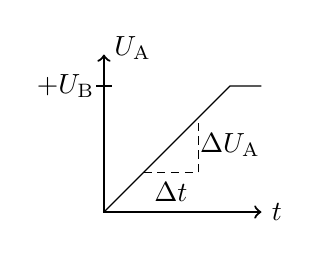
\begin{tikzpicture}
        \draw[thick,->] (-0.015,0) -- (2,0) node[anchor=west] {$t$};
        \draw[thick,->] (0,0) -- (0,2) node[anchor=south west, pos=0.9] {$U_\mathrm{A}$};
        \draw (0,0) -- (1.6,1.6) -- (2,1.6);
        \draw[thick] (-0.1,1.6) -- (0.1,1.6);
        \draw (0,1.6) node[anchor=east] {$+U_\mathrm{B}$};
        
        \draw[densely dashed] (0.5,0.5) -- (1.2,0.5) -- ++(0,0.7);  % Steigungsdreieck Linien
            \node at (1.6,0.85) {$\Delta U_\mathrm{A}$};
            \node at (0.85,0.25) {$\Delta t$}; 
    \end{tikzpicture}
}  &
            Slew rate: $\frac{\Delta U_A}{\Delta t}$           &
            \scalebox{0.8}{    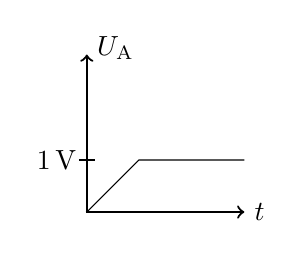
\begin{tikzpicture}
        \draw[thick,->] (-0.015,0) -- (2,0) node[anchor=west] {$t$};
        \draw[thick,->] (0,0) -- (0,2) node[anchor=south west, pos=0.9] {$U_\mathrm{A}$};
        \draw (0,0) -- (0.66,0.66) -- (2,0.66);
        \draw[thick] (-0.1,0.66) -- (0.1,0.66) node[anchor=east, pos=0.5] {$1\,\mathrm{V}$};
    \end{tikzpicture}
}  &
            \scalebox{0.8}{    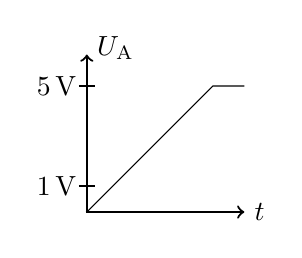
\begin{tikzpicture}
        \draw[thick,->] (-0.015,0) -- (2,0) node[anchor=west] {$t$};
        \draw[thick,->] (0,0) -- (0,2) node[anchor=south west, pos=0.9] {$U_\mathrm{A}$};
        \draw (0,0) -- (1.6,1.6) -- (2,1.6);
        \draw[thick] (-0.1,0.33) -- (0.1,0.33) node[anchor=east, pos=0.5] {$1\,\mathrm{V}$};
        \draw[thick] (-0.1,1.6) -- (0.1,1.6) node[anchor=east, pos=0.5] {$5\,\mathrm{V}$};
    \end{tikzpicture}}    \\
            \hline
        \end{tabular}
        \caption{Verschaltung eines Verstärkers als Komparator (A), Impedanzwandler (C) und nicht-invertierender Verstärker (D)}
        \label{fig: Verschaltung Verstaerker}
    \end{figure}

    %\fu{
    %    \resizebox{\textwidth}{!}{\input{Tikz/src/Verschaltungdesverstaerkers.tex}}
    %    }{Verschaltung eines Verstärkers als Komparator (A), Impedanzwandler (C) und nicht-invertierender Verstärker (D)
    %    \label{fig: Verschaltung Verstaerker}}

    \speech{Gegenkopplung_Bsp_Lsg_3}{1}{Wenn wir noch zwei Widerstände verbauen, führen wir nur einen Teil der Ausgangsspannung zurück an den invertierenden Eingang. Das Ergebnis: Wir können die Verstärkung der Schaltung mit den Widerständen einstellen. Die Formel lautet: V gleich eins plus  R zwei geteilt durch R eins. Das ist der klassische nichtinvertierende Verstärker. Damit lässt sich unser Lautsprecherproblem elegant lösen: Wir brauchen nur die passenden Widerstände.}
    %seed: 875701
    \silence{3}
\end{frame}


\begin{frame}
    \s{
        \begin{bsp}{Teil 2: Entwicklung einer Verstärkerschaltung für Musiksignale}{Beispiel Verstaerkung 2}
            Im letzten Schritt muss ermittelt werden, wie die Widerstände in (D) gewählt werden müssen, damit sich eine Verstärkung von 10 ergibt. Dazu müssen zunächst die Maschengleichungen aufgestellt werden.
            Eine wichtige Annahme zur Aufstellung dieser Maschengleichung ist, dass davon ausgegangen wird, dass der Verstärker durch die Rückkopplung des Ausgangsignal die beiden Eingangssignale angleicht.
            Hier darf also geschrieben werden \glqq Annahme: $U_{\textnormal{dif}}=0$~V\grqq{}.
            Somit ergibt sich für den invertierenden Eingang $U_{\textnormal{E-}}=1\,\mathrm{V}$.
            Da weiterhin davon ausgegangen wird, dass kein Strom in die Eingänge hineinfließt gilt $I_{\textnormal{R1}}~=~I_{\textnormal{R2}}$.
            Die Maschengleichung lautet auf Grundlage dieser Annahmen
            \begin{equation}
                U_{\textnormal{A}} = U_{\textnormal{R1}} + U_{\textnormal{R2}} = U_{\textnormal{E}} + I_{\textnormal{R2}} \cdot R_{\textnormal{2}} = U_{\textnormal{E}} + \frac{U_{\textnormal{E}}}{R_{\textnormal{1}}} \cdot R_{\textnormal{2}}
            \end{equation}
    
            Dadurch ergibt sich das Ein-Ausgangsverhalten im zeitbereich zu folgendem Ausdruck.
            \begin{equation}
                \frac{U_{\textnormal{A}}}{U_{\textnormal{E}}} = \underbrace{(1+\frac{R_2}{R_1})}_{V}
            \end{equation}
    
    
            Wird diese Gleichung nach $R_2/R_1$ gelöst, ergibt sich das Verhältnis der Widerstände für das oben beschriebene
            Problem zu $R_2/R_1 = 9$. Die Widerstände sollten hier nicht zu groß gewählt werden, da dann der Ausgleichsstrom zwischen
            Ausgang und Eingang zu klein werden könnte. Das kann zu einem starken Rauschen am Verstärkerausgang führen. Übliche Widerstandswerte sind in der Regel den Beispielschaltungen des Datenblattes eines
            Operationsverstärkers zu entnehmen. In diesem Fall könnte z.B. $R_2=9~\textnormal{k}\Omega$ und $R_1=1~\textnormal{k}\Omega$ gewählt werden.
        \end{bsp}
    
        \par
        Ähnnlich wie für die oben dargestellte Schaltung lassen sich auch für alle weiteren Operationsverstärkerschaltungen Übertragungsfunktionen herleiten. Das soll hier allerdings nicht gezeigt werden.
        Weitere Übertragungsfuktionen für einige ausgewählte Operationsverstärkergrundschaltungen können Tabelle \ref{tab:Grundschaltungen} entnommen werden.
        In dieser Tabelle sind die die Schaltungen, die Bodediagramme mit Phasengang (rot) und Amplitudengang (blau) und die Übertragungsfunktionen angegeben.
        Nachdem nun die Beschaltung von Verstärkern vorgestellt wurde, soll im Folgenden Kapitel nun noch eine wichtige Eigenschaft von Verstärkerschaltungen thematisiert werden, die sich aus den genutzen Verstärkerbausteinen und der äußeren Verschaltung ergibt: Die Stabilität der Verstärkerschaltung.
    
        \begin{block}{}
            \input{Bilder/kap3/Frequenzgang_verschiedener_Opvs.tex}
            %\label{OPV Schaltungen Tabelle}
            %\caption{Tabelle mit ausgewählten Operationsverstärkerschaltungen}
        \end{block}
        %\label{fig:Frequenzgang OPVs}
    }

    \b{
        \frametitle{Prinzip der Gegenkopplung - Lösung des Beispielproblems (3)}
        \begin{columns}
            \column[c]{0.3\textwidth}
            \begin{center}
                \scalebox{0.8}{    \begin{circuitikz}
        \ctikzset{tripoles/en amp/input height=-0.45}
        \draw (0,0) node[en amp](E){};
        \draw (E.+) to[open, o-, v, name=Ud] (E.-);
        \draw (E.-) to [short, o-*] ++(0, -1.25) coordinate(ref);
        \draw (E.out) to[short, *-] ++(ref -| 0,0) 
            to[R, l_=$R_2$, i>_, v^, name=R2] (ref)
            to[R, l=$R_1$, i, v, name=R1] ++(0, -1.75)
            node[ground]{} coordinate(ref1);
        \draw (E.out) to[short, -o] ++(0.25,0) node[right]{$U_\mathrm{A}$}
            to[open, -o, v^, name=Ua] ++(ref1 -| 0,0) node[ground]{};
 
        \varrmore{R1}{$U_\mathrm{R1}$};
        \varrmore{R2}{$U_\mathrm{R2}$};
        \iarrmore{R1}{$I_\mathrm{R1}$};
        \iarrmore{R2}{$I_\mathrm{R2}$};
        \varrmore{Ud}{$U_\mathrm{Diff}=0\,\mathrm{V}$};
        \varrmore{Ua}{$U_\mathrm{A}$};
    \end{circuitikz} }
                Finale Verstärkerschaltung mit Rückführung
                \label{fig:Verschaltung des Verstärkers2}
            \end{center}
            \column[c]{0.6\textwidth}
            Annahme: $U_{\textnormal{Diff}}$~=~0
            \onslide<1->{
                \begin{equation}
                    U_\mathrm{A} = U_\mathrm{R1} + U_\mathrm{R2} = U_\mathrm{E} + I_\mathrm{R2} \cdot R_2
                \end{equation}}
            \onslide<2->{
                \begin{equation}
                    U_\mathrm{A} = U_\mathrm{E} + \frac{U_\mathrm{E}}{R_1} \cdot R_2
                \end{equation}}
            \onslide<3->{
                \begin{equation}
                    \frac{U_\mathrm{A}}{U_\mathrm{E}} = \underbrace{(1+\frac{R_2}{R_1})}_{V_{Gain}}
                \end{equation}}
            \onslide<3->{
                Weitere OPV-Grundschaltungen sind Skript zu finden.}
        \end{columns}
    }
 \end{frame}

%Folie Nichtinvertierender Verstärker
\begin{frame}
    \b{
        \frametitle{Nichtinvertierender Verstärker}
        \begin{columns}
            \column{0.3\textwidth}
            \centering
            \begin{figure}
                \centering
                \begin{subfigure}{\linewidth}
                    \centering
                    \scalebox{1}{\input{Tikz/src/NichtinvertierenderVerstaerker.tex}}
                    \caption{Schaltung eines nichtinvertierenden Verstärkers}
                \end{subfigure}
                \begin{subfigure}{\linewidth}
                    \centering
                    \scalebox{0.7}{\input{Tikz/src/FrequenzgangNiV.tex}}
                    \caption{Frequenzgang eines nichtinvertierenden Verstärkers}
                \end{subfigure}
            \end{figure}

            \column{0.6\textwidth}
            \begin{itemize}
                \item Gleichung:
                      \[
                          U_{\textnormal{A}} = \left(1+\frac{R_2}{R_1}\right) U_{\textnormal{E}}
                      \]
                \item Phasengleiches Ausgangssignal
                \item Sehr hochohmiger Eingangswiderstand
                \item Niederohmiger Ausgangswiderstand
                \item Anwendungen: z.B. Impedanzwandler
            \end{itemize}
        \end{columns}
    }
    \speech{Grundschaltungen_NIV}{1}{Hier sehen wir die Standardbeschaltung. Das Eingangssignal liegt am nichtinvertierenden Eingang. Ein Teil der Ausgangsspannung wird über R1 und R2 zurückgeführt. Eigenschaften dieser Schaltung sind folgende: Die Ausgangsspannung ist phasengleich zum Eingang. Der Eingangswiderstand ist sehr hoch, der Ausgangswiderstand sehr niedrig. Die Verstärkung lässt sich sauber über R1 und R2 einstellen und mit der unten abgebildeten Formel berechnen. Typische Anwendungen sind Impedanzwandler oder einfache Verstärker mit hoher Eingangsimpedanz.}
    %seed: 877869
    \silence{3}
\end{frame}

\begin{frame}
    \b{
        \frametitle{Invertierender Verstärker}
        \begin{columns}
            \column{0.3\textwidth}
            \centering
            \begin{figure}
                \centering
                \begin{subfigure}{\linewidth}
                    \centering
                    \scalebox{1}{\input{Tikz/src/InvertierenderVerstaerker.tex}}
                    \caption{Schaltung eines invertierenden Verstärkers}
                \end{subfigure}
                \begin{subfigure}{\linewidth}
                    \centering
                    \scalebox{0.7}{\input{Tikz/src/FrequenzgangInvertierenderVerstaerker.tex}}
                    \caption{Frequenzgang eines invertierenden Verstärkers}
                \end{subfigure}
            \end{figure}

            \column{0.6\textwidth}
            \begin{itemize}
                \item Gleichung:
                      \[
                          U_{\textnormal{A}} = \frac{R_2}{R_1} U_{\textnormal{E}}
                      \]
                \item -180$^\circ$ Phasenverschiebung zwischen Ein- zu Ausgang
                \item $R_1$ bestimmt den Eingangswiderstand
                \item Niederohmiger Ausgangswiderstand
                \item Anwendungen: z.B. Aktiver Spannungsteiler zum Messen hoher Spannungen, wenn $R_1 > R_2$
            \end{itemize}
        \end{columns}
    }
    \speech{Grundschaltungen_IV}{1}{Jetzt das Gegenstück: der invertierende Verstärker. Hier legen wir das Eingangssignal über einen Widerstand R1 direkt an den invertierenden Eingang. Am nichtinvertierenden Eingang liegt Masse. Eigenschaften dieser Schaltung: Die Ausgangsspannung ist um hundertachtzig Grad phasenverschoben - also invertiert. Der Verstärkungsfaktor ist V gleich minus R2  geteilt durch R1. Die Eingangsimpedanz entspricht R1. Das macht die Schaltung sehr gut geeignet als aktiver Spannungsteiler.}
    %seed: 896223 
    \silence{3}
\end{frame}


\begin{frame}
    \b{
        \frametitle{Komparator}
        \begin{columns}
            \column{0.3\textwidth}
            \centering
            \begin{figure}
                \centering
                \begin{subfigure}{\linewidth}
                    \centering
                    \scalebox{1}{\input{Tikz/src/Komparator.tex}}
                    \caption{Schaltung eines Komparators}
                \end{subfigure}
                \begin{subfigure}{\linewidth}
                    \centering
                    \scalebox{0.7}{\input{Tikz/src/FrequenzgangKomparator.tex}}
                    \caption{Frequenzgang eines Komparators}
                \end{subfigure}
            \end{figure}

            \column{0.6\textwidth}
            \begin{itemize}
                \item Gleichung:
                      \[
                          V_1: U_{\textnormal{E+}} > U_{\textnormal{E-}} \Rightarrow U_{\textnormal{A}} \approx +U_{\textnormal{B}}
                      \]
                      \[
                          V_2: U_{\textnormal{E+}} < U_{\textnormal{E-}} \Rightarrow U_{\textnormal{A}} \approx -U_{\textnormal{B}}
                      \]
                \item Einsatz in Zweipunktreglern und Analog-Digital-Wandlern
            \end{itemize}
        \end{columns}
    }
    \speech{Grundschaltungen_KOMP}{1}{Hier nochmal der Komparator zum Vergleich. Er vergleicht die Spannungen am Plus- und  Minus-Eingang: Ist U E plus größer, geht der Ausgang auf plus U B. Ist U E minus größer, geht er auf minus U B. Das Prinzip findet man zum Beispiel bei Zweipunktreglern oder in der Analog-Digital Wandlung.} 
    %seed: 896323 
    \silence{3}
\end{frame}


\begin{frame}
    \b{
        \frametitle{Summierer}
        \begin{columns}
            \column{0.3\textwidth}
            \centering
            \begin{figure}
                \centering
                \begin{subfigure}{\linewidth}
                    \centering
                    \scalebox{1}{\input{Tikz/src/Summierer.tex}}
                    \caption{Schaltung eines Summierers}
                \end{subfigure}
                \begin{subfigure}{\linewidth}
                    \centering
                    \scalebox{0.7}{\input{Tikz/src/FrequenzgangSummierer.tex}}
                    \caption{Frequenzgang eines Summierers}
                \end{subfigure}
            \end{figure}

            \column{0.6\textwidth}
            \begin{itemize}
                \item Gleichung:
                      \[
                          U_{\textnormal{A}} = \underbrace{\frac{R_3} {R_1}}_{V_1} \cdot U_{\textnormal{E1}} + \underbrace{\frac{R_3} {R_2}}_{V_2} \cdot U_{\textnormal{E2}}
                      \]
                \item Der Summierer basiert auf dem invertierenden Verstärker und findet Verwendung in Analogrechnern und beim Mischen von Spannungssignalen
            \end{itemize}
        \end{columns}
    }
    \speech{Grundschaltungen_SUM}{1}{Mit O P Vaus können wir auch mehrere Signale addieren. Dazu legen wir die Eingangssignale über Widerstände auf den invertierenden Eingang. Der O P Vau sorgt dann dafür, dass die Summenspannung am Ausgang entsteht. So entstehen Addierer-Schaltungen, die in Analogrechnern oder Mischpulten verwendet werden.}
    %seed: 896345 
    \silence{3}
\end{frame}


\begin{frame}
    \b{
        \frametitle{Subtrahierer}
        \begin{columns}
            \column{0.3\textwidth}
            \centering
            \begin{figure}
                \centering
                \begin{subfigure}{\linewidth}
                    \centering
                    \scalebox{1}{\input{Tikz/src/Subtrahierer.tex}}
                    \caption{Schaltung eines Subtrahierers}
                \end{subfigure}
                \begin{subfigure}{\linewidth}
                    \centering
                    \scalebox{0.7}{\input{Tikz/src/FrequenzgangSubtrahierer.tex}}
                    \caption{Frequenzgang eines Subtrahierers}
                \end{subfigure}
            \end{figure}

            \column{0.6\textwidth}
            \raggedleft
            \begin{itemize}
                \item Gleichung:
                      \[
                          {U_A} = {U_{{\textnormal{E2}}}} \cdot \underbrace{ \frac{R_1 + R_2}{R_1} \cdot \frac{R_4}{R_3 + R_4}}_{V_2} - U_{\textnormal{E1}} \cdot \underbrace{\frac{R_2}{R_1}}_{V_1}
                      \]
                \item Wenn alle Widerstände gleich groß sind, wird die Differenz der Signale $U_{E1}$ und $U_{E2}$ gebildet, weswegen diese Schaltung als Differenzverstärker bezeichnet wird
            \end{itemize}
        \end{columns}
    }
    \speech{Grundschaltungen_SUB}{1}{Ganz ähnlich können wir Signale auch subtrahieren. Das passiert in einer Schaltung, die oft auch Differenzverstärker genannt wird. Wenn alle Widerstände gleich groß sind, dann gilt: U A gleich in Klammern U 2 minus U 1 mal Verstärkung Diese Schaltung ist besonders wichtig, wenn wir kleine Differenzsignale aus großen Gleichtaktstörungen herausziehen wollen.}
    %seed: 896347
    \silence{3}
\end{frame}



\begin{frame}
    \b{
        \frametitle{Integrierer}
        \begin{columns}
            \column{0.3\textwidth}
            \centering
            \begin{figure}
                \centering
                \begin{subfigure}{\linewidth}
                    \centering
                    \scalebox{1}{\input{Tikz/src/Integrierer.tex}}
                    \caption{Schaltung eines Integrierers}
                \end{subfigure}
                \begin{subfigure}{\linewidth}
                    \centering
                    \scalebox{0.55}{\input{Tikz/src/FrequenzgangIntegrierer.tex}}
                    \caption{Frequenzgang eines Integrierers}
                \end{subfigure}
            \end{figure}

            \column{0.6\textwidth}
            \raggedleft
            \begin{itemize}
                \item Gleichung:
                      \[
                          U_A(t) = - \frac{R_2}{R_1} U_{\textnormal{E}}(t) - \int_0^t \frac{U_{\textnormal{E}}(t)}{R_1 C_1} \, dt
                      \]
                \item Nimmt eine Integration des Eingangssignals vor
                \item Wird als aktives Tiefpassfilter verwendet
            \end{itemize}
        \end{columns}
    }
    \speech{Grundschaltungen_INT}{1}{Eine weitere wichtige Grundschaltung ist der Integrierer. Im Rückkopplungszweig liegt parallel zum Widerstand ein Kondensator. Das Ergebnis: Am Ausgang erscheint das Integral des Eingangssignals. So können wir zum Beispiel aus einem Rechtecksignal ein Dreiecksignal machen. In der Signalverarbeitung ist das auch die Grundlage für aktive Tiefpassfilter.}
    %seed: 896349
    \silence{3}
\end{frame}


\begin{frame}
    \b{
        \frametitle{Differenzierer}
        \begin{columns}
            \column{0.3\textwidth}
            \centering
            \begin{figure}
                \centering
                \begin{subfigure}{\linewidth}
                    \centering
                    \scalebox{1}{\input{Tikz/src/Differenzierer.tex}}
                    \caption{Schaltung eines Differenzierers}
                \end{subfigure}
                \begin{subfigure}{\linewidth}
                    \centering
                    \scalebox{0.7}{\input{Tikz/src/FrequenzgangDifferenzierer.tex}}
                    \caption{Frequenzgang eines Differenzierers}
                \end{subfigure}
            \end{figure}

            \column{0.6\textwidth}
            \raggedleft
            \begin{itemize}
                \item Gleichung:
                      \begin{align*}
                          U_{\textnormal{A}}(t) =
                          &- \frac{R_2}{R_1} \, U_{\textnormal{E}}(t)
                          - \int_0^t \frac{1}{R_1 C_1} \, U_{\textnormal{E}}(\tau) \, d\tau\\
                          &- R_2 C_2 \, \frac{dU_{\textnormal{E}}}{dt}(t)
                      \end{align*}
                \item Nimmt eine Differenziation des Eingangssignals vor
                \item Wird als aktives Hochpassfilter verwendet (zeigt in der Realität meist Bandpassverhalten, wie hier dargestellt)
            \end{itemize}
        \end{columns}
    }
    \speech{Grundschaltungen_DIFF}{1}{Der umgekehrte Fall ist der Differenzierer. Jetzt liegt im Eingang noch ein Kondensator. Das Ergebnis: Am Ausgang erscheint die Ableitung des Eingangssignals. Ein Rechtecksignal am Eingang wird so zu scharfen Spannungsspitzen am Ausgang. Die Schaltung zeigt also ein Hochpassverhalten. Praktisch verwendet man oft Varianten, die eher wie ein Bandpass arbeiten, um Rauschen zu vermeiden.}
    %seed: 885433
    \silence{3}
\end{frame}


\begin{frame}
    \b{
        \frametitle{Logarithmierer}
        \begin{columns}
            \column{0.3\textwidth}
            \centering
            \begin{figure}
                \centering
                \input{Tikz/src/Logarithmierer.tex}
                \caption{Schaltung eines Logarithmierers}
            \end{figure}

            \column{0.6\textwidth}
            \raggedleft
            \begin{itemize}
                \item Gleichung:
                      \[
                          U_{\textnormal{A}} =-U_{\textnormal{T}}\cdot \ln{\left(\frac{U_{\textnormal{E}}}{R_1\cdot I_S}\right)}
                      \]
                      \[
                          U_{\textnormal{T}} = \frac{\textnormal{k}_{\textnormal{B}} \cdot T}{\textnormal{e}}
                      \]

                      \(\textnormal{e} = \text{Elementarladung}\)

                      \(\textnormal{k}_{\textnormal{B}} = \text{Boltzmannkonstante}\)

                      \(I_{\textnormal{s}} = \text{Sperrstrom der Diode}\)
                \item Bildet den natürlichen Logarithmus des Eingangssignals
            \end{itemize}
        \end{columns}
    }
    \speech{Grundschaltungen_LOG}{1}{Noch spannender wird es, wenn wir eine Diode in den Rückkopplungszweig legen. Dann bildet der OP V die logarithmische Kennlinie der Diode nach. Das heißt: Am Ausgang steht die logarithmierte Eingangsspannung. Solche Schaltungen braucht man zum Beispiel bei Signalaufbereitung oder in Analogrechnern.}
    %seed: 885433  
    \silence{3}
\end{frame}

\begin{frame}
    \b{
        \frametitle{Potenzierer}
        \begin{columns}
            \column{0.3\textwidth}
            \centering
            \begin{figure}
                \centering
                {\input{Tikz/src/Potenzierer.tex}}
                \caption{Schaltung eines Potenzierers}
            \end{figure}

            \column{0.6\textwidth}
            \raggedleft
            \begin{itemize}
                \item Gleichung:
                      \[
                          U_{\textnormal{A}} =-R_1\cdot I_{\textnormal{S}} \cdot e^{\frac{U_{\textnormal{E}}}{U_{\textnormal{T}}}}
                      \]
                \item Besitzt einen e-funktionalen Zusammenhang zwischen Ein- und Ausgangsspannung
            \end{itemize}
        \end{columns}
    }
    \speech{Grundschaltungen_POT}{1}{Ähnlich können wir mit Dioden oder Transistoren auch eine exponentielle Kennlinie aufbauen. Dann ergibt sich am Ausgang ein Signal, das eine Potenzfunktion oder eine e-Funktion des Eingangssignals darstellt. Auch das war in klassischen Analogrechnern ein zentrales Werkzeug.}
        %seed: 885434 
    \silence{3}
\end{frame}

\begin{frame}
    \b{
        \frametitle{Instrumentenverstärker}
        \begin{columns}
            \column{0.3\textwidth}
            \centering
            \begin{figure}
                \centering
                \begin{subfigure}{\linewidth}
                    \centering
                    \scalebox{1}{\input{Tikz/src/Instrumentenverstaerker.tex}}
                    \caption{Schaltung eines Instrumentenverstärkers}
                \end{subfigure}
                \begin{subfigure}{\linewidth}
                    \centering
                    \scalebox{0.7}{\input{Tikz/src/FrequenzgangInstrumenten.tex}}
                    \caption{Frequenzgang eines Instrumentenverstärkers}
                \end{subfigure}
            \end{figure}

            \column{0.6\textwidth}
            \raggedleft
            \begin{itemize}
                \item Gleichung:
                      \[
                          \mathit{a_i} : \text{Amplitude Eingangsspannung i}
                      \]
                      \[
                          \mathit{\varphi_i} : \text{Phase Eingangsspannung i}
                      \]
                      \[
                          \mathit{A}_{A} = \sqrt{a_1^2 + a_2^2 + 2a_1a_2 \cos(\varphi_1 - \varphi_2)}
                      \]
                      \[
                          \mathit{\tan}(\varphi_A) = \frac{a_1 \mathit{\sin}(\varphi_1) + a_2 \mathit{\sin}(\varphi_2)}{a_1 \mathit{\cos}(\varphi_1) + a_2 \mathit{\cos}(\varphi_2)}
                      \]
                      \[
                          \text{Wenn} : R_2 = R_4 = R
                      \]
                      \[
                          U_{\textnormal{A}} = (1+ \frac{2R} {R_{\textnormal{g}}}) \cdot \frac{R_3} {R_2} (U_{\textnormal{E2}}-U_{\textnormal{E1}})
                      \]
                \item Differenzverstärker mit hoher Eingangsimpedanz und hoher Gleichtaktunterdrückung
            \end{itemize}
        \end{columns}
    }
    \speech{Grundschaltungen_IA}{1}{Hier sehen wir einen Instrumentenverstärker. Das ist im Prinzip ein sehr präziser Differenzverstärker, bei dem die Eingangsstufe hochohmig ist und die Verstärkung über einen einzigen Widerstand eingestellt werden kann. Die große Stärke: Er unterdrückt Gleichtaktsignale sehr gut - ideal, um zum Beispiel kleine Sensorsignale aus verrauschten Umgebungen herauszufiltern.}
    %seed: 885435 
    \silence{3}
\end{frame}


\begin{frame}
    \b{
        \frametitle{Impedanzwandler}
        \begin{columns}
            \column{0.3\textwidth}
            \centering
            \begin{figure}
                \centering
                \scalebox{.6}{\input{Tikz/src/Impedanzwandler.tex}}
                \caption{Schaltung eines Impedanzwandlers}
            \end{figure}

            \column{0.6\textwidth}
            \centering
            \begin{itemize}
                \item Ausgangsspannung $U_\mathrm{A}$ folgt der Eingangsspannung $U_\mathrm{E}$
                \item Verstärkung $V = \frac{U_\mathrm{A}}{U_\mathrm{E}} = 1$
                \item Auch Spannungsfolger genannt
                \item Hoher Eingangswiderstand durch Operationsverstärker
                \item Typische Anwendung: Sensoren
            \end{itemize}
        \end{columns}
    }
    \speech{Grundschaltungen_Imp}{1}{Zum Schluss nochmal der Impedanzwandler, manchmal auch Spannungsfolger genannt. Hier wird der Ausgang direkt mit dem invertierenden Eingang verbunden, während das Eingangssignal auf den nichtinvertierenden Eingang gelegt wird. Das Ergebnis: Die Ausgangsspannung entspricht genau der Eingangsspannung. Der Eingangswiderstand ist extrem hoch, der Ausgangswiderstand extrem niedrig. Damit eignet sich diese Schaltung hervorragend als Pufferstufe - sie belastet die Quelle nicht, kann aber selbst größere Ströme liefern.}
    %seed: 885464 
    \silence{3}
\end{frame}